\section{Organisation usuelle d'un projet d'annotation}
\label{section:2.2-ORGANISATION-ANNOTATION}
	
	%%% Introduction: 
	Dans la section précédente, nous avons présenté l'importance d'avoir des données annotées pour entraîner d'un modèle de \textit{Machine Learning}.
	Maintenant, nous allons détailler la préparation et l'organisation de cette tâche d'annotation, et identifier les compétences nécessaires aux intervenants du projet.
	
	
	%%%
	%%% Subsection 2.2.1: Étapes clés du cycle d'annotation.
	%%%
	\subsection{Étapes clés du cycle d'annotation}
	\label{section:2.2.1-ORGANISATION-ANNOTATION-ETAPES-CLES}
		% \cite{pustejovsky-stubbs:2012:natural-language-annotation} et \cite{stubbs:2013:methodology-using-professional} formalisation MATTER
		
		%%% Introduction au cycle MATTER.
		Une référence en matière d'organisation de projet d'annotation est proposé par \cite{pustejovsky-stubbs:2012:natural-language-annotation} : les auteurs y formalisent la conception et l'amélioration \textbf{cyclique} d'un modèle de \textit{Machine Learning}.
		Ce cycle est appelé cycle \texttt{MATTER} en référence aux six étapes de conception qui le composent : \textit{\textbf{M}odelize}, \textit{\textbf{A}nnotate}, \textit{\textbf{T}rain}, \textit{\textbf{T}est}, \textit{\textbf{E}valuate} et \textit{\textbf{R}evise}.
		Ces étapes sont schématisées en \textsc{Figure~\ref{figure:2.2.1-ORGANISATION-ANNOTATION-ETAPES-CLES-MATTER}} et nous détaillons chacune d'entre elles ci-dessous.
		%
		\begin{figure}[!htb]
			\centering
			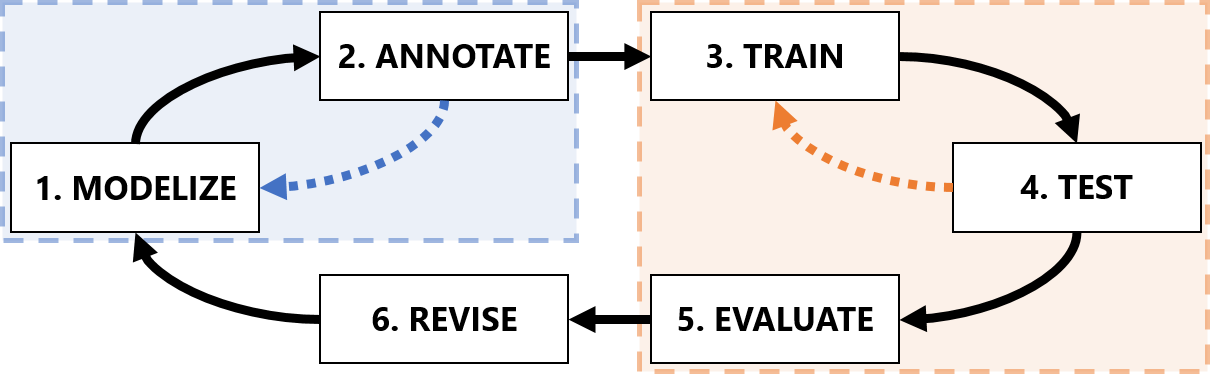
\includegraphics[width=0.95\textwidth]{figures/etatdelart-pustejovsky-2012-cycle-matter-mama-tt}
			\caption{
				Cycle \texttt{MATTER} structurant un projet d'annotation en six étapes principales: \textit{\textbf{M}odelize}, \textit{\textbf{A}nnotate}, \textit{\textbf{T}rain}, \textit{\textbf{T}est}, \textit{\textbf{E}valuate} et \textit{\textbf{R}evise}.
			}
			\label{figure:2.2.1-ORGANISATION-ANNOTATION-ETAPES-CLES-MATTER}
		\end{figure}
		
		%%% 2.2.1.A. Concevoir la base d'apprentissage (\textbf{M}odelize}, \textit{\textbf{A}nnotate}).
		\subsubsection{Concevoir la base d'apprentissage (\textit{\textbf{M}odelize}, \textit{\textbf{A}nnotate}).}
		\label{section:2.2.1.A-ORGANISATION-ANNOTATION-ETAPES-CLES-MODELIZE-ANNOTATE}
		
			%%% a. Collecte de données.
			Pour obtenir un bon modèle de \textit{Machine Learning}, il faut avoir une base d’apprentissage de qualité.
			Comme nous l'avons dit précédemment, cela commence par disposer d'un ensemble de données d'exemples qui représente fidèlement les différentes facettes du problème à modéliser.
			Une phase de \texttt{collecte} de données est alors organisée : cette collecte peut se baser sur des extractions de bases de données ou de sites internet à disposition, sur des enquêtes réalisées après d'utilisateurs finaux, ou encore sur les avis éclairés d'experts du problème.
			Ces données brutes ont ensuite besoin d'être annotées pour pouvoir être exploitées. \\
			
			%%% b. Modelisation des données.
			
			% Importance de la modélisation.
			Afin de garantir la qualité de cette labellisation, \textbf{il est important de ne pas précipiter la tâche d'annotation}.
			En effet, l'objectif de cette tâche et les informations nécessaires à annoter sur chaque données peuvent considérablement changer en fonction du phénomène à décrire, des données à disposition et de la finalité du modèle de \textit{Machine Learning} à entraîner.
			Il est donc fortement conseillé de bien \textbf{modéliser le problème} pour clarifier les attendus et les modalités de cette annotation (voir \textsc{Figure~\ref{figure:2.2.1-ORGANISATION-ANNOTATION-ETAPES-CLES-MATTER}}, étape 1. \textit{\textbf{M}odelize}).
			
			% Modélisation vs Spécification, Guide d'annotation et exemple.
			\cite{pustejovsky-stubbs:2012:natural-language-annotation} distinguent ici deux concepts importants de cette phase :
			\begin{itemize}
				\item la \textbf{modélisation} du problème, représentation de manière abstraite l'objectif à atteindre et décrivant ainsi la logique générale de l'annotation dans un \textit{schéma d'annotation} ;
				\item les \textbf{spécifications}, compilant dans un \textit{guide d'annotation} l'ensemble des règles concrètes à respecter pour mettre en application la modélisation.
			\end{itemize}
			Pour résumer cette distinction, la modélisation représente \textit{quoi} annoter (\textit{objectif, définition, valeurs possibles, ...}) alors que les spécifications décrivent \textit{comment} annoter (\textit{règles d'attribution, exemples et contre-exemple, règles de format, ...}).
			\begin{leftBarExamples}
				% Exemple littérature.
				\cite{perrotin-etal:2018:annotation-actes-dialogue}, s'intéressant à la classification des conversations d'assistance en ligne en actes de dialogues, décrit son guide d'annotation dans \cite{asher-etal:2017:manuel-annotation-actes}.
				On y retrouve (1) la modélisation avec la présentation des étiquettes possibles à annoter, et (2) les spécifications avec les définitions concrètes, des exemples, des restrictions d'attribution, et la gestion des données non pertinentes. \\
				% Exemple BD.
				Dans nos exemples précédents (cf. \textsc{Section~\ref{section:2.1.2.B-PRESENTATION-ANNOTATION-EXEMPLES-CLASSIFICATION}}), nous avions modélisé le problème de classification de l'état d'une bande dessinée en quatre classes : "\texttt{Mauvais état}", "\texttt{Bon état}", "\texttt{Très bon état}", "\texttt{Neuf}".
				Il faudrait désormais rédiger les spécifications avec des définitions concrètes et quelques exemples  pour guider un annotateur, notamment pour l'aider à distinguer "\texttt{Bon état}" de "\texttt{Très bon état}".
			\end{leftBarExamples}
			
			% Quelques points importants sur la modélisation et exemples.
			Bien entendu, il n'est pas toujours facile de modéliser un problème ni de rédiger un guide d'annotation adéquat.
			Nous reviendrons plus tard sur les caractéristiques de cette tâche pouvant introduire de la complexité (voir \textsc{Section~\ref{section:2.3-DEFIS-ANNOTATION}}), mais il est important de souligner d'emblée les points élémentaires suivants :
			\begin{itemize}
				\item le besoin d'\textit{inter-opérabilité} et de \textit{ré-utilisabilité} : un projet d'annotation est toujours un investissement coûteux, il serait donc regrettable de perdre ou de ne pas pourvoir ré-utiliser ces données après ce projet.
				Par conséquent, il faut réfléchir au format des données ainsi qu'aux types de détails à fournir pour être sûr de pouvoir toujours exploiter les données si la modélisation évolue légèrement ou si un futur projet désire en bénéficier ;
				\item la balance entre \textit{généralité} et \textit{spécificité} : le niveau de détail requis dépend sans conteste du problème à modéliser : annoter trop peu de détail ne permet pas d'exploiter les données, mais en annoter trop peut rapidement complexifier la tâche et introduire des erreurs.
				Il faut donc trouver le juste milieu pour réaliser un travail de qualité qui ne soit pas trop pénible.
			\end{itemize}
			\begin{leftBarExamples}
				Dans la classification de langue exposée en \textsc{Section~\ref{section:2.1.2.B-PRESENTATION-ANNOTATION-EXEMPLES-CLASSIFICATION}}, nous y avons annoté chaque texte grâce à trois classes : "\texttt{Français}", "\texttt{Anglais}" et "\texttt{Allemand}".
				\begin{itemize}
					% Exemple inter-opérabilité et de ré-utilisabilité.
					\item par soucis d'\textit{inter-opérabilité}, nous pourrions plutôt utiliser la norme ISO 639-3 (\cite{international-organization-for-standardization:2007:codes-representation-names}), soit les code "\texttt{fra}", "\texttt{eng}" et "\texttt{deu}", afin de standardiser l'annotation et ainsi pouvoir partager plus facilement les données labellisées avec d'autres projets ;
					% Exemple généralité et spécificité.
					\item afin de présenter un cas simple, nous avions proposé un modèle avec trois langues communes pour une bande dessinée d'origine belge.
					Toutefois, nous aurions pu \textit{spécialiser} davantage notre modèle en fonction des variations régionales en prenant en compte le Corse ("\texttt{cos}") ou le Wallon ("\texttt{wln}").
					Cette distinction peut être essentielle pour certaines saga publiées dans ces langues (comme \texttt{Astérix \& Obélix}), mais peut simplement être une source de confusion pour les autres (comme \texttt{Lucky Luke}).
				\end{itemize}
			\end{leftBarExamples}
			
			
			%%% c. Annotation
			
			% Annotation en tant que telle.
			Lorsque le guide d'annotation est rédigé, la \textbf{phase de labellisation} peut commencer (voir \textsc{Figure~\ref{figure:2.2.1-ORGANISATION-ANNOTATION-ETAPES-CLES-MATTER}}, étape 2. \textit{\textbf{A}nnotate}).
			Cette tâche est traditionnellement réalisée par un groupe d'experts choisi en fonction de leur connaissance du problème à caractériser (dans nos exemples sur les bandes dessinées, ce serait plutôt des libraires ou des collectionneurs).
			Après leur avoir expliqué l'objectif de leur travail et partagé les règles de labellisation contenues dans le guide, les annotateurs se partagent les données et réalisent chacun une partie du corpus d'apprentissage.
			
			%%% d. Mini-cycle MAMA.
			
			\begin{leftBarInformation}
				% La théorie rencontre le réel.
				C'est généralement à ce stade que la théorie rencontre la pratique : certaines règles d'annotation peuvent difficilement être applicables, certains données peuvent être ambiguës ou hors-sujet, et deux annotateurs peuvent aussi avoir des avis différents sur l'annotation la plus adéquate.
				\cite{pustejovsky-stubbs:2012:natural-language-annotation} introduisent donc le premier sous-cycle \texttt{MAMA} en référence à la boucle entre \textit{\textbf{M}odelize} et \textit{\textbf{A}nnotate} qui peut avoir lieu tant que le guide d'annotation n'est pas adapté aux données manipulées.
				
				% Exemple.
				Par exemple, lors de l'annotation de la transcription audio en \textsc{Section~\ref{section:2.1.2.D-PRESENTATION-ANNOTATION-EXEMPLES-TRANSCRIPTION}}, il peut y avoir une voix principale accompagnée de plusieurs voix en arrière plan : une première adaptation du guide serait de clarifier si ces voix secondaires doivent être transcrites ou ignorées, voire si l'audio entier doit être considéré comme inexploitable.
				La réponse à cette question dépend bien entendu du phénomène à décrire et de l'objectif du modèle de \textit{Machine Learning} à entraîner : dans notre cas, nous pourrions probablement annoter uniquement la voix principale et ignorer l'audio si le bruit gène la compréhension.
			\end{leftBarInformation}
			
			%%% Finalité : la base d'apprentissage.
			À la fin de l'annotation (ou du cycle \texttt{MAMA}), le corpus d'entraînement est disponible pour concevoir un modèle de \textit{Machine Learning}.
			
		
		%%% 2.2.1.B. Concevoir le modèle (\textit{\textbf{T}rain}, \textit{\textbf{T}est}, \textit{\textbf{E}valuate}).
		\subsubsection{Concevoir le modèle (\textit{\textbf{T}rain}, \textit{\textbf{T}est}, \textit{\textbf{E}valuate}).}
		\label{section:2.2.1.B-ORGANISATION-ANNOTATION-ETAPES-CLES-TRAIN-TEST}
			
			%%% Apprentissage statistiques et importance du test.
			La phase d'entraînement du modèle est l'étape centrale de l'apprentissage automatique.
			Toutefois, comme l'apprentissage se base sur des méthodes statistiques, il est important d'introduire une phase de test et d'évaluation pour s'assurer des performances du modèle obtenu.
			Il est donc courant de considérer une boucle de raffinement du modèle tant que les performances n'ont pas atteint un seuil acceptable (voir \textsc{Figure~\ref{figure:2.2.1-ORGANISATION-ANNOTATION-ETAPES-CLES-MATTER}}, étapes 3. \textit{\textbf{T}rain}, 4. \textit{\textbf{T}est} et 5. \textit{\textbf{E}valuate}).
			
			%%% Train/Dev/Test.
			En pratique, il est d'usage de \textbf{créer trois jeux de données} à partir de la base d'apprentissage qui vient d'être annotée :
			\begin{itemize}
				\item le jeu d'\texttt{entraînement}: c'est sur cette partie des données que le modèle de \textit{Machine Learning} est conçu ;
				\item le jeu de \texttt{développement} (ou de validation): le modèle entraîné est évalué sur ce jeu de donnée pour étudier son comportement, identifier ses forces et ses faiblesses, et ainsi permettre de le comparer à d'autres modèles entraînés pour cette même tâche ;
				\item le jeu de \texttt{test} : le modèle retenu est évalué sur ce jeu de test pour déterminer ses performances réelles. Il est important que ce jeu de données 
			\end{itemize}
			% [van-der-goot:2021:we-need-talk]: définir un train/tune/dev/test
			
			%%% Evaluate.
			Ainsi, le modèle représente la connaissance présente dans le jeu \texttt{entraînement}, il est étudié puis affiné grâce au jeu de \texttt{développement}, et est finalement jugé en fonction de ses performances sur le jeu de \texttt{test}.
			Il est encore une fois difficile d'être exhaustif sur les analyses et les métriques à considérer car elles dépendent fortement du type de problème que le modèle tente de résoudre.
			Une métrique basique est l'\texttt{Accuracy} (ou taux de bonne prédiction), décrivant simplement le nombre de fois que le modèle a fait une bonne proposition sur l'ensemble du test.
			Suivant le problème et le type de données, d'autres métriques usuelles peuvent être utilisées comme le \texttt{MSE} (\textit{Mean Squared Error}) pour la prédiction de variables numérique (voir \cite{wallach-goffinet:1987:mean-squared-error}), le \texttt{f1-score} pour les variables catégorielles (voir \cite{sasaki:2007:truth-fmeasure}) ou le \texttt{WER} (\textit{Word Error Rate}) pour la transcription de textes (voir \cite{mccowan-etal:2005:use-information-retrieval}).
			Dans tous les cas, une règle d'or est de bien tenir à l'écart le jeu de test des deux autres jeux de données et qu'il ne soit pas utilisé dans la phase de développement pour éviter tout biais de sur-apprentissage\footnote{Pour plus de détails sur le sur-apprentissage: voir \cite{collins:2017:chapter-overfitting}}.

			%%% Finalité : le modèle et se sperformances.
			À la fin de ce cycle, le modèle de \textit{Machine Learning} est disposition à l'emploi, et ses performances théoriques sont celles obtenues sur le jeu de test.
		
		%%% 2.2.1.C. Revoir la base d'apprentissage (\textit{\textbf{R}evise}).
		\subsubsection{Revoir la base d'apprentissage (\textit{\textbf{R}evise}).}
		\label{section:2.2.1.C-ORGANISATION-ANNOTATION-ETAPES-CLES-REVISE}
		
			% Besoin de réviser.
			Pour terminer cette boucle, il est parfois nécessaire d'envisager de corriger son modèle en remettant en cause la modélisation du problème et l'annotation des données.
			\cite{voormann-gut:2008:agile-corpus-creationa} formalisait en effet ce besoin de réviser la conception d'une base d'apprentissage en observant les lacunes du modèle obtenu, et \cite{pustejovsky-stubbs:2012:natural-language-annotation} évoque certaines révisions nécessaires de la modélisation dès la phase d'annotation (voir sous-cycle \texttt{MAMA} dans la \textsc{Figure~\ref{figure:2.2.1-ORGANISATION-ANNOTATION-ETAPES-CLES-MATTER}}).
			
			% Identifier un besoin de réviser.
			Divers pistes peuvent mener à une évolution de la base d'apprentissage :
			\begin{itemize}
				\item le modèle de \textit{Machine Learning} peut avoir de mauvaise performances, malgré son affinage lors de la phase de développement, ou peut manquer d'adaptabilité sur des données réelles ;
				\item la modélisation ou l'annotation peuvent devenir obsolète car le phénomène modélisé évolue dans le temps ;
				\item un cas d'usage non identifié jusqu'à présent nécessite de nouvelles données pour être pris en compte ;
				\item ou encore, un nouvel algorithme de \textit{Machine Learning} a priori plus performat requiert une modélisation différente pour traiter le problème.
			\end{itemize}
			\begin{leftBarExamples}
				% Exemple Inflation prix
				Pour illustrer nos propos, prenons la tâche d'estimation du prix d'une bande dessinée (cf. \textsc{Section~\ref{section:2.1.2.A-PRESENTATION-ANNOTATION-EXEMPLES-REGRESSION}}) : il se peut que les prix annoté sur les transactions ne soient plus d'actualité à cause de l'inflation, et que les données doivent être ré-annotées pour prendre en compte les nouvelles valeurs du marché.
				
				% Exemple ajouter une classe.
				D'autre part, la modélisation en tant que telle peut aussi être impacté : par exemple, dans le cadre de la classification de l'état d'une bande dessinée à partir d'une photo (cf. \textsc{Section~\ref{section:2.1.2.B-PRESENTATION-ANNOTATION-EXEMPLES-CLASSIFICATION}}), on pourrait constater à l'usage qu'il manque une catégorie "\texttt{Très mauvais état}" nécessaire pour trier d’emblée toute \texttt{BD} indigne à la vente.
				
				% Exemple OCR.
				Enfin, il est possible que le modèle se comporte mal sur certaines données.
				Par exemple lors de l'identification d'une bande dessinée à partir de sa couverture (cf. \textsc{Section~\ref{section:2.1.2.C-PRESENTATION-ANNOTATION-EXEMPLES-EXTRACTION}}), certains textes du décors pourrait être extrait à tord (comme le texte de la pancarte \textguillemets{\textit{Saloon}} dans la \textsc{Figure~\ref{figure:2.1.2.C-PRESENTATION-ANNOTATION-EXEMPLES-EXTRACTION}}).
				Il faudra peut-être adapter l'annotation pour identifier les textes à ne pas extraire (avec une classe de rebus par exemple).
			\end{leftBarExamples}
			
			% Conclusion.
			Nous bouclons ainsi le cycle \texttt{MATTER} qui préfigure le besoin d'amélioration continue de tout modèle de \textit{Machine Learning}.
			
	
	%%%
	%%% Subsection 2.2.2: Portraits des acteurs intervenant sur un projet d'annotation.
	%%%
	\subsection{Portraits des acteurs intervenant sur un projet d'annotation}
	\label{section:2.2.2-ORGANISATION-ANNOTATION-ACTEURS}
		\todo[inline]{SECTION: À RÉDIGER: \\
			- Acteurs: Objectifs, Rôles, Compétences, ... ; \\
			~~~~ - Axe métier (business expert) ; \\
			~~~~ - Axe technique (data scientist) ; \\
			~~~~ - Axe manipulation (data analyst) ; \\
			~~~~ - Axe projet (project leader) ;
			% [fort:2017:experts-ou-foule] caractérise trois types d’expert :
				% du domaine du corpus (médical, juridique, politique),
				% du domaine de l’annotation (sémantique, transcription de l’oral, syntaxique),
				% de la tâche
			% choix / formation d'annotateurs (experts métiers, pas des experts en IA ou en annotation)
				% minimum 2 pour engager des débats
				% [bayerl-paul:2011:what-determines-intercoder] : plus on est nombreux, moins on est d'accord
		}

% [stubbs:2013:methodology-using-professional]
% For example, the following list of guideline users is paraphrased/restructured from Dipper et al. (2004a):
% > The annotator: Annotators apply the annotation specification (the tags and attributes) to the chosen corpus by following the annotation guideline instructions. Interests: the goal of the annotation, and how to apply the annotation specification to the corpus.
% > The corpus explorer : Explorers are interested in using the corpus to examine linguistic theories. Interests: how to find examples of linguistic phenomena and interpret the annotation, information about the corpus itself.
% > The language engineer : Engineers want to use automatic methods to explore the corpus and annotations; for example: through extracting linguistic information through evaluation scripts, or using the corpus to train machine learning algorithms. Interests: tagsets, corpus creation methods.
% > The guideline explorer: The annotation guidelines themselves are of interest to linguists who want to understand the theory behind the annotation, or people who want to create their own guidelines for a different annotation task. Interests: guideline creation and underlying theory.
% > The guideline author: Because guidelines often have to be revised multiple times before a task, the guideline authors themselves will often need to refer back to their own work to ensure the coverage of the guidelines is complete. Interests: clear organization of instructions.
% >It should be noted that Dipper et al. (2004a) use the term 'guidelines' to refer to all the information relevant to researchers, including information about the corpus, the linguistic theory, the annotation, and so on, while this dissertation uses the traditional definition of `guidelines', as described at the beginning of this section.
% >However, despite this terminological difference, Dipper et al. make excellent points about the information that should be made available when an annotated corpus is released to the public based on the different interests of various types of researchers. Another recent study by Bayerl and Paul (2011) examined what factors in an annotation task may in uence inter-annotator agreement (IAA) scores.
	
	
	%%%
	%%% Subsection 2.2.3: Exemples de logiciels utilisés pour annoter.
	%%%
	\subsection{Exemples de logiciels utilisés pour annoter}
	\label{section:2.2.3-ORGANISATION-ANNOTATION-LOGICIELS}
		\todo[inline]{SECTION: À RÉDIGER: \\
			% [finlayson-erjavec:2016:overview-annotation-creation]: tools
			- Outils: Liste, Avantages, Inconvénients, Fonctionnalités ;
			~~~~ - Excel
			~~~~ - prodigy
				% - Glozz [Widlöcher & Mathet, 2009] http://www.glozz.org/
				% - Callisto [Day et al., 2004]
				% - MMAX2 [Müller, 2006] https://github.com/ottiram/MMAX2
				% - PALinkA [Orăsan, 2003]
				% - Gate [Cunningham_2022] https://gate.ac.uk/
				% - Brat [Stenetorp et al., 2012] http://brat.nlplab.org/
				% - WebAnno [Yimam et al., 2013] https://webanno.github.io/webanno/
				% - Inception [Klie et al., 2018] https://inception-project.github.io/
		}
	
	
	% Conclusion.
	\begin{leftBarSummary}
		\begin{todolist}
			\item[\itemok] Un projet d'annotation s'organise généralement en cycle (\texttt{MATTER}) au cours duquel l'annotateur créé une modélisation abstraite des données, définit ses règles d'annotation, réalise sa labellisation, puis entraîne son modèle. Il peut être amené à réviser sa modélisation des données en fonction des performances obtenues.
			\item[\itemok] Un tel projet d'annotation nécessite une diversité de connaissances et de compétences (\textit{connaissances métiers, connaissances techniques, maîtrise de l'apprentissage automatique, ...}), faisant ainsi collaborer un grand nombre d'acteurs qualifiés pour une ou plusieurs phase du cycle d'annotation.
		\end{todolist}
	\end{leftBarSummary}